%%%%%%%%%%%%%%%%%%%%%%%%%%%%%%%%%%%%%%%%%%%%%%%%%%%%%%%%%%%%
%%% LaPreprint: PREPRINT TEMPLATE
%%%%%%%%%%%%%%%%%%%%%%%%%%%%%%%%%%%%%%%%%%%%%%%%%%%%%%%%%%%%

%%%%%%%%%%%%%%%%%%%%%%%%%%%%%%%%%%%%%%%%%%%%%%%%%%%%%%%%%%%%
%%% PREAMBLE
%%%%%%%%%%%%%%%%%%%%%%%%%%%%%%%%%%%%%%%%%%%%%%%%%%%%%%%%%%%%

% Declare document class
\documentclass[12pt,biorxiv,lineno,doublespacing]{lapreprint}

% Import packages
\usepackage[version=4]{mhchem} % For chemical notation
\usepackage{siunitx}    % For SI units
\usepackage{pdflscape}  % For putting pages in landscape mode
\usepackage{rotating}   % For rotating specific elements
\usepackage{textgreek}  % Greek symbols
\usepackage{gensymb}    % Symbols
\usepackage[misc]{ifsym} % For the \Letter symbol
\usepackage{orcidlink}  % For the \orcidlink
\usepackage{listings}   % For inserting code chunks
\usepackage{colortbl}   % For Knitr table colouring
\usepackage{tabularx}   % For making Knitr tables compatible
\usepackage{longtable}  % For multi-page tables
\usepackage{threeparttable}
\usepackage{subcaption}
\usepackage{multirow}
\usepackage{snotez}     % For sidenote environments. enotez for endnotes
\usepackage{csquotes}   % For language-based quote rules (helps BiBLaTeX)
\usepackage{setspace}
\usepackage{fontenc}
\usepackage{cleveref}
\usepackage{makecell}

% Make declarations
\DeclareSIUnit\Molar{M}

%%%%%%%%%%%%%%%%%%%%%%%%%%%%%%%%%%%%%%%%%%%%%%%%%%%%%%%%%%%%
%%% BIBLIOGRAPHY
%%%%%%%%%%%%%%%%%%%%%%%%%%%%%%%%%%%%%%%%%%%%%%%%%%%%%%%%%%%%
\usepackage[			% use biblatex for bibliography
	backend=biber,      % use biber or bibtex backend
    style=authoryear,   % choose style
	natbib=true,		% allow natbib commands
	hyperref=true,	    % activate hyperref support
	alldates=year,      % only show year (not month)
]{biblatex}

% Update to your bibliography file
\addbibresource{src/references.bib}

%%%%%%%%%%%%%%%%%%%%%%%%%%%%%%%%%%%%%%%%%%%%%%%%%%%%%%%%%%%%
%%% ARTICLE SETUP
%%%%%%%%%%%%%%%%%%%%%%%%%%%%%%%%%%%%%%%%%%%%%%%%%%%%%%%%%%%%

% Paper title
\title{Functional MRI brain state occupancy in the presence of cerebral small vessel disease -- pre-registration for a multiverse replication analysis of the Hamburg City Health Study}

% Authors - you can use \orcidlink{} and \authfn{} - see contribution note
\author[ \orcidlink{0000-0002-5729-2935} 1 \Letter]{Eckhard Schlemm, MBBS PhD}
%\author[ \orcidlink{0000-0003-2434-1822} 1 \authfn{1}]{Bastian Cheng, MD}

% Affiliations
\affil[1]{Department of Neurology, University Medical Center Hamburg-Eppendorf}

% Correspondence
\correspondence{e.schlemm@uke.de}{}

% Contribution note
%\contribution[\authfn{1}]{These authors contributed equally.}

% Present address of corresponding author
\presentaddress[]{\\Dr.\, Dr.\, Eckhard Schlemm, Klinik und Poliklinik f\"ur Neurologie, Universit\"atsklinikum Hamburg-Eppendorf, Martinistr. 52,\\ D-20251 Hamburg}

% Data availability statement, funding and competing interests.
\data[]{Preprocessed data will be available e.g. on \href{https://github.com/csi-hamburg/HCHS-brain-states-RR}{https://github.com/csi-hamburg/HCHS-brain-states-RR}.}
\funding[]{Deutsche Forschungsgemeinschaft (DFG) -- 178316478 -- C2}
\compint[]{The author declares no competing interests.}


% Surname of the lead author(s) for the running footer
\leadauthor{Eckhard Schlemm}
\shorttitle{Brain states in cSVD - a functional MRI replication substudy of the Hamburg City Health Study}


%%%%%%%%%%%%%%%%%%%%%%%%%%%%%%%%%%%%%%%%%%%%%%%%%%%%%%%%%%%%
%%% ARTICLE START
%%%%%%%%%%%%%%%%%%%%%%%%%%%%%%%%%%%%%%%%%%%%%%%%%%%%%%%%%%%%

\begin{document}
\maketitle

\begin{abstract}

{\bf Objective:} To replicate recent findings on the association between the extent of cerebral small vessel disease (cSVD), functional brain network dedifferentiation, and cognitive impairment.

{\bf Methods:} We analyzed demographic, imaging, and behavioral data from the prospective population-based Hamburg City Health Study.
Using a fully prespecified analysis pipeline, we estimated discrete brain states from structural and resting-state functional magnetic resonance imaging (MRI).
In a multiverse analysis, we varied brain parcellations and functional MRI confound regression strategies.
The severity of cSVD was operationalized as the volume of white matter hyperintensities of presumed vascular origin.
Processing speed and executive dysfunction were quantified using the Trail Making Test (TMT).

{\bf Hypotheses:} We hypothesized a) that a greater volume of supratentorial white matter hyperintensities would be associated with less time spent in functional MRI-derived brain states of high fractional occupancy;
and b) that less time spent in these high-occupancy brain states is associated with a longer time to completion in part B of the TMT. 

{\bf Results:} High-occupancy brain states were characterized by activation or suppression of the default mode network. 
Every \num{5.1}-fold increase in WMH volume was associated with a \num{0.94}-fold reduction in the odds of occupying DMN-related brain states (P \num{5.01e-8}). Every \qty{5}{\percent} increase in time spent in high-occupancy brain states was associated with a \num{0.98}-fold reduction in the TMT-B completion time (P \num{0.0116}). 
Findings were robust across most brain parcellations and confound regression strategies.

{\bf Conclusion:} We successfully replicated previous findings on the association between cSVD, functional brain occupancy, and cognition in an independent sample. 
The data provide further evidence for a functional network dedifferentiation hypothesis of cSVD-related cognitive impairment. 
Further research is required to elucidate the mechanisms underlying these associations. 
\end{abstract}


\section{Introduction} \label{intro}
Cerebral small vessel disease (cSVD) is an arteriolopathy of the brain, associated with age and common cardiovascular risk factors \citep{Wardlaw2013-yd}.
cSVD predisposes to ischemic, in particular lacunar, stroke and may lead to cognitive impairment and dementia \citep{Cannistraro2019-ly}.
Neuroimaging findings in cSVD reflect its underlying pathology \citep{Wardlaw2015-ri} and include white matter hyperintensities (WMH) and lacunes of presumed vascular origin, small subcortical infarcts and microbleeds, enlarged perivascular spaces as well as brain atrophy \citep{Wardlaw2013-sc}.
However, the extent of visible cSVD features on magnetic resonance imaging (MRI) is an imperfect predictor of the severity of clinical sequelae \citep{Das2019-pc}, and our understanding of the causal mechanisms linking cSVD-associated brain damage to clinical deficits remains limited \citep{Bos2018-qj}.

Recent efforts have concentrated on exploiting network aspects of the structural \citep{Tuladhar2016-ae,Tuladhar2020-fp,Lawrence2018-ti} and functional \citep{Dey2016-qg,Schulz2021-ho} organization of the brain to understand the relation between cSVD and clinical deficits in cognition and other domains reliant on distributed processing.
Reduced structural network efficiency has repeatedly been described as a causal factor in the development of cognitive impairment, in particular executive dysfunction, in cSVD \citep{Lawrence2014-xp,Shen2020-yv,Reijmer2016-wm,Prins2005-ej}.
Findings with respect to functional connectivity results, on the other hand, are more heterogeneous, perhaps due to its limited reproducibility in the presence of cSVD and dependence on arbitrary processing choices \citep{Lawrence2018-sv,Gesierich2020-db}.
As a promising new avenue, time-varying, or dynamic, functional connectivity approaches have more recently been explored in patients with subcortical ischemic vascular disease \citep{Yin2022-cv,Xu2021-ib}.

In the present paper, we aim to replicate and extend the main results of \citep{Schlemm2022-he};
in this recent study, the authors analyzed MR imaging and clinical data from the prospective Hamburg City Health Study (HCHS, \citep{Jagodzinski2020-lx}) using a coactivation pattern approach to define discrete brain states and found associations between the WMH load, time spent in high-occupancy brain states characterized by activation or suppression of the default mode network (DMN) and executive dysfunction.

Our primary hypothesis is that the volume of supratentorial white matter hyperintensities is associated with the fractional occupancy (defined below) of DMN-related brain states in a middle-aged to elderly population mildly affected by cSVD.
Our second hypothesis is that this fractional occupancy is associated with executive dysfunction, measured as the time to complete part B of the trail making test (TMT).

Both hypotheses will be tested in an independent subsample of the HCHS study population using the same imaging protocols, examination procedures and analysis pipelines as in \citep{Schlemm2022-he}.
The robustness of associations will be explored in a multiverse approach by varying key steps in the analysis pipeline.

\section{Methods} \label{methods}

\subsection{Study population}
The paper will analyze data from the Hamburg City Health Study (HCHS), which is an ongoing prospective, population-based cohort study aiming to recruit a cross-sectional sample of \num{45000} adult participants from the city of Hamburg, Germany \citep{Jagodzinski2020-lx}.
From the first \num{10000} participants of the HCHS we will aim to include those who were documented to have received brain imaging (n=2652) and exclude those who were analyzed in our previous report \citep{Schlemm2022-he}.
The ethical review board of the Landesärztekammer Hamburg (State of Hamburg Chamber of Medical Practitioners) approved the HCHS (PV5131), all participants provided written informed consent.

\subsection{Demographic and clinical characterization}
From the study database we will extract participants’ age at the time of inclusion in years, their self-reported gender and the number of years spent in education.
During the visit at the study center, participants undergo cognitive assessment using standardized tests.
We will extract from the database their performance scores in the Trail Making Test part B, measured in seconds, as an operationalization of executive function \citep{Tombaugh2004-dp}.

\subsection{MRI acquisition and preprocessing}
The magnetic resonance imaging protocol for the HCHS includes structural and resting-state functional sequences.
The acquisition parameters on a \qty{3}{\tesla} Siemens Skyra MRI scanner (Siemens, Erlangen, Germany) have been reported before \citep{Petersen2020-cx,Frey2021-sv} and are given as follows:

For $T_1$-weighted anatomical images, a 3D rapid acquisition gradient-echo sequence (MPRAGE) was used with the following sequence parameters: repettion time $\text{TR} = \qty{2500}{\ms}$, echo time $\text{TE} = \qty{2.12}{\ms}$, 256 axial slices, slice thickness $\text{ST} = \qty{0.94}{\mm}$, and in-plane resolution  $\text{IPR} = \qtyproduct[product-units = bracket-power]{0.83 x 0.83}{\mm}$.

$T_2$-weighted fluid attenuated inversion recovery (FLAIR) images were acquired with the following sequence parameters: $\text{TR} = \qty{4700}{\ms}$, $\text{TE} = \qty{392}{\ms}$, \num{192} axial slices, $\text{ST} = \qty{0.9}{\mm}$, $\text{IPR} = \qtyproduct[product-units = bracket-power]{0.75 x 0.75}{\mm}$.

\num{125} resting state functional MRI volumes were acquired ($\text{TR} = \qty{2500}{\ms}$; $\text{TE} = \qty{25}{\ms}$; $\text{flip angle} = \ang[]{90}$; slices = \num{49}; $\text{ST} = \qty{3}{\mm}$; $\text{slice gap} = \qty{0}{\mm}$; $\text{IPR} = \qtyproduct[product-units = bracket-power]{2.66 x 2.66}{\mm}$).
Subjects were asked to keep their eyes open and to think of nothing.

We will verify the presence and voxel-dimensions of expected MRI data for each participant and exclude those for whom at least one of $T_1$-weighted, FLAIR and resting-state MRI is missing.
To ensure reproducibility, no visual quality assessment on raw images will be performed.

For the remaining participants, structural and resting-state functional MRI data will be preprocessed using FreeSurfer v6.0 (\url{https://surfer.nmr.mgh.harvard.edu/}), and fmriPrep v20.2.6 \citep{Esteban2019-sx}, using default parameters. Participants will be excluded if automated processing using at least one of these packages fails.

\subsection{Quantification of WMH load}
For our primary analysis, the extent of ischemic white matter disease will be operationalized as the total volume of supratentorial WMHs obtained from automated segmentation using a combination of anatomical priors, BIANCA \citep{Griffanti2016-dt} and LOCATE \citep{Sundaresan2019-ww}, post-processed with a minimum cluster size of \num{30} voxels, as described in \citep{Schlemm2022-he}.
In an exploratory analysis, we partition voxels identified as WMH into deep and periventricular components according to their distance to the ventricular system (cut-off $\qty{10}{\mm}$, \citep{Griffanti2018-oa})

\subsection{Brain state estimation}
Output from fMRIprep will be post-processed using xcpEngine v1.2.1 to obtain de-confounded spatially averaged BOLD time series \citep{Ciric2017-cl}.
For the primary analysis we will use the \textit{36p} regression strategy and the Schaefer-\num{400} parcellation \citep{Schaefer2018-bo}, as in \citep{Schlemm2022-he}.
 
Different atlases and confound regression strategies, as implemented in xcpEngine, will be included in the exploratory multiverse analysis.

Co-activation pattern (CAP) analysis will be performed by first aggregating parcellated, de-confounded BOLD signals into a $\left(n_{\text{parcels}}\times \sum_i{n_{\text{time points}, i}}\right)$ feature matrix, where $n_{\text{time points}, i}$ denotes the number of retained volumes for subject $i$ after confound regression.
Clustering will be performed using the $k$-means algorithm ($k=5$) with distance measure given by 1 minus the sample Pearson correlation between points, as implemented in Matlab R2021a.
We will estimate subject- and state-specific fractional occupancies, which are defined as the proportion of BOLD volumes assigned to each brain state \citep{Vidaurre2018-pb}. 
The two states with the highest average occupancy will be identified as the basis for further analysis.


\subsection{Statistical analysis}
For demographic (age, gender, years of education) and clinical (TMT-B) variables the number of missing records will be reported.
For non-missing values, we will provide descriptive summary statistics using median and interquartile range.
The proportion of men and women in the sample will be reported.

As a first outcome-neutral quality check of the implementation of the MRI processing pipeline, brain state estimation and co-activation pattern analysis, we will compare fractional occupancies between brain states.
We expect that the average fractional occupancy in two high-occupancy states is higher than the average fractional occupancy in the other three states.
Point estimates and 95\% confidence intervals will be presented for the difference in average fractional occupancy to check this assertion.

For further analyses, non-zero WMH volumes will be subjected to a logarithmic transformation.
Zero values will retain their value zero; to compensate, all models will include a binary indicator for zero WMH volume if at least one non-zero value is present.

To assess the primary hypothesis of a negative association between the extent of ischemic white matter disease and time spent in high-occupancy brain states, we will perform a fixed-dispersion beta-regression to model the logit of the conditional expectation of the average fractional occupancy of two high-occupancy states as an affine function of the logarithmized WMH load.
Age and gender will be included as covariates.
The strength of the association will be quantified as an odds ratio per interquartile ratio of the WMH burden distribution and accompanied by a 95\% confidence interval.
Significance testing of the null hypothesis of no association will be conducted at the conventional significance level of 0.05.
Estimation and testing will be carried out using the 'betareg' package v3.1.4 in R v4.2.1.

To  assess the secondary hypothesis of an association between time spent in high-occupancy brain states and executive dysfunction, we will perform a generalized linear regression with a Gamma response distribution to model the logarithm of the conditional expected completion time in part B of the TMT as an affine function of the average fractional occupancy of two high-occupancy states.
Age, gender, years of education and logarithmized WMH load will be included as covariates.
The strength of the association will be quantified as a multiplicative factor per percentage point and accompanied by a 95\% confidence interval.
Significance testing of the null hypothesis of no association will be conducted at the conventional significance level of 0.05.
Estimation and testing will be carried out using the glm function included in the 'stats' package from R v4.2.1.

Sample size calculation is based on the data presented in \citep{Schlemm2022-he}, where an odds ratio of \qty{0.95} was reported as the primary effect size of interest.
We used simple bootstrapping to create \num{10000} hypothetical datasets of size \num{200}, \num{400}, \num{600}, \num{800}, \num{900}, \num{910}, \ldots, \num{1100}, \num{1200}, \num{1400}, \num{1500}, \num{1600}.
Each dataset was subjected to the estimation procedure described above.
For each sample size, the proportion of datasets in which the primary null hypothesis of no association between fractional occupancy and WMH load could be rejected at $\alpha=0.05$ was computed and is recorded as a power curve in \Cref{fig:power}.

\begin{figure}
    \includegraphics[width=.5\linewidth]{./../analysis/code/R/pipeline_files/figure-html/power-1.png}
    \caption{Estimated power for different sample sizes is obtained as the proportion of synthetic data sets in which the null hypothesis of no association between WMH volume and time spent in high-occupancy brain states an be rejected at the $\alpha=0.05$ significance level. Proportions are based on a total of \num{10000} synthetic data sets obtained by bootstrapping the data presented in \citep{Schlemm2022-he}. Highlighted in orange are the smallest sample size ensuring a power of at least \qty{80}{\percent} ($n=960$), the sample size of the pilot data ($n=988$, post-hoc power \qty{81.3}{\percent}), and the expected sample sample size for this replication study ($n=1500$, a-priori power \qty{93.9}{\percent}).}
    \label{fig:power}
\end{figure}

It is seen that a sample size of \num{960} would allow replication of the reported effect with a power of \qty{80.2}{\percent}.
We anticipate a sample size of \num{1500}, which yields a power of \qty{93.9}{\percent}.


\subsection{Multiverse analysis}
Both in \citep{Schlemm2022-he} and for our primary replication analysis we made certain analytical choices in the operationalisation of brain states and ischemic white matter disease, namely the use of the \textit{36p} confound regression strategy, the Schaefer-\num{400} parcellation and a BIANCA/LOCATE-based WMH segmentation algorithm.
If the hypothesized association between WMH burden and time spent in high-occupancy states can be replicated using these primary analytical choices, its robustness with regard to other choices will be explored in a multiverse analysis \citep{Schlemm2022-he,Steegen2016-ze}.
Specifically, we will estimate brain states from BOLD time series processed according to a variety of established confound regression strategies and aggregated over different cortical brain parcellations (\Cref{tab:multiverse}, \cite{ciric2018mitigating,Ciric2017-cl}). Extent of cSVD will additionally be quantified by the volume of deep and periventricular white matter hyperintensities.

\renewcommand\cellset{\renewcommand\arraystretch{0.5}%
    \setlength\extrarowheight{0pt}}
\begin{table}[bt]
    \begin{threeparttable}
        \begin{subtable}[t]{.75\textwidth}
            \label{tab:parcellations2}
            % Use "S" column identifier to align on decimal point 
            \begin{tabularx}{\textwidth}{l l l}
                \toprule
                \textbf{Name of the atlas}  & \textbf{\#parcels}                                  & \textbf{Reference}          \\
                \midrule
                Desikan--Killiany           & \num{86}                                            & \cite{desikan2006automated} \\
                AAL                         & \num{116}                                           & \cite{tzourio2002automated} \\
                Harvard--Oxford             & \num{112}                                           & \cite{makris2006decreased}  \\
                glasser360                  & \num{360}                                           & \cite{Glasser2016-ia}       \\
                gordon333                   & \num{333}                                           & \cite{Gordon2016-wy}        \\
                power264                    & \num{264}                                           & \cite{Power2011-xf}         \\
                schaefer\{N\}               & \makecell[lt]{\num{100} \\ \num{200}\\ \num{400}}   & \cite{Schaefer2018-bo}      \\
                \bottomrule
            \end{tabularx}
            \begin{tablenotes}
                \item{AAL:} Automatic Anatomical Labelling
            \end{tablenotes}
            \caption{Parcellations}
        \end{subtable}
        \qquad
        \begin{subtable}[t]{.75\textwidth}
            \label{tab:parcellations}
            % Use "S" column identifier to align on decimal point 
            \begin{tabularx}{\textwidth}{l l l}
                \toprule
                \textbf{Design}        & \textbf{Reference}                 \\
                \midrule
                24p                    & \cite{friston1996movement}         \\
                24p + GSR              & \cite{macey2004method}             \\
                36p              & \cite{satterthwaite2013improved}   \\
                36p + spike regression & \cite{cox1996afni}                 \\
                36p + despiking        & \cite{satterthwaite2013improved}   \\
                36p + scrubbing  & \cite{power2014methods}            \\
                aCompCor               & \cite{muschelli2014reduction}      \\
                tCompCor               & \cite{behzadi2007component}        \\
                AROMA                  & \cite{pruim2015ica}                \\
                \bottomrule
            \end{tabularx}
            \begin{tablenotes}
                \item GSR: Global signal regression, AROMA: Automatic Removal of Motion Artifacts
            \end{tablenotes}
            \caption{Confound regression strategies, adapted from \citep{Ciric2017-cl}}
        \end{subtable}
        \makeatletter\def\TPT@hsize{}\makeatletter
    \end{threeparttable}
    \mycaption{Multiverse analysis}{Overview over different brain parcellations and confound regression strategies implemented using xcpEngine \citep{ciric2018mitigating}. A total of $9\times 9=81$ analytical combinations were explored to assess the robustness of our results with respect to these processing choices.}
    \label{tab:multiverse}
\end{table}

For each combination of analytical choice of confound regression strategy, parcellation and subdivision of white matter lesion load ($9\times9\times3=243$ scenarios in total) we will quantify the association between WMH load and average time spent in high-occupancy brain states using odds ratio and \qty{95}{\percent} confidence intervals as described above.
No hypothesis testing and, therefore, no adjustment for multiple testing, will be carried out in these non-primary analyses.

\section{Exploratory analysis}
In previous work, two high-occupancy brain states were related to the default-mode network \citep{Cornblath2020-fu}.
We will further explore this relation by computing, for each individual brain state, the cosine similarity of the positive and negative activations of the cluster’s centroid with a set of a-priori defined functional ‘communities’ or networks \citep{Schaefer2018-bo,Yeo2011-qg}.
Results will be thus visualized as spider plots for the Schaefer, Gordon and Power atlasses.


\section{Code and pilot data}
Summary data from the first \num{1000} imaging data points of the HCHS have been published with \citep{Schlemm2022-he}  and form the basis for the hypotheses tested in this replication study.
We have implemented our prespecified analysis pipeline described above in R and Matlab, and applied it to this previous sample.
Data, code and results have been stored on GitHub (\url{https://github.com/csi-hamburg/HCHS_brain_states_RR}) und preserved on Zenodo.

Thus re-analysing data from \num{988} subjects, the separation between two high-occupancy and three low-occupancy brain states could be reproduced for all combinations of brain parcellation and confound regression strategies (\Cref{fig:separation}).

\begin{figure}
    \includegraphics[width=\linewidth]{./../analysis/code/R/pipeline_files/figure-html/highVSlowFOplot-1.png}
    \caption{Point estimates (dots) and \qty{95}{\percent} confidence intervals (line segments) for the mean difference in fractional occupancy between high- and low occupancy states are shown for different confound regression strategies (groups along the vertical axis) and brain parcellations (color). 
    The difference in FO for a particular choice of regression strategy and brain parcellation is nominally statistically significantly different from zero at a significance level of 5\% if the corresponding interval does not contain zero. Hence, the FO difference is significant for \emph{all} processing choices, reflecting the separation between high- und low-occupancy states.
    The primary choices (\textit{36p} and \textit{schaefer400}) are highlighted by a yellow box and thick pink line, respectively. The effect size reported in \citep{Schlemm2022-he} is indicated by a vertical line at 0.08830623.}
    \label{fig:separation}
\end{figure}

In a multiverse analysis, the main finding was somewhat robust with respect to these choices: a statistically significant negative association between WMH load and time spent in high-occupancy states was observed in 18/81 scenarios, with 5/81 statistically significant positive associations occurring with the Desikan--Killiany parcellation only (\Cref{fig:refWMHvsFO}).

\begin{figure}
    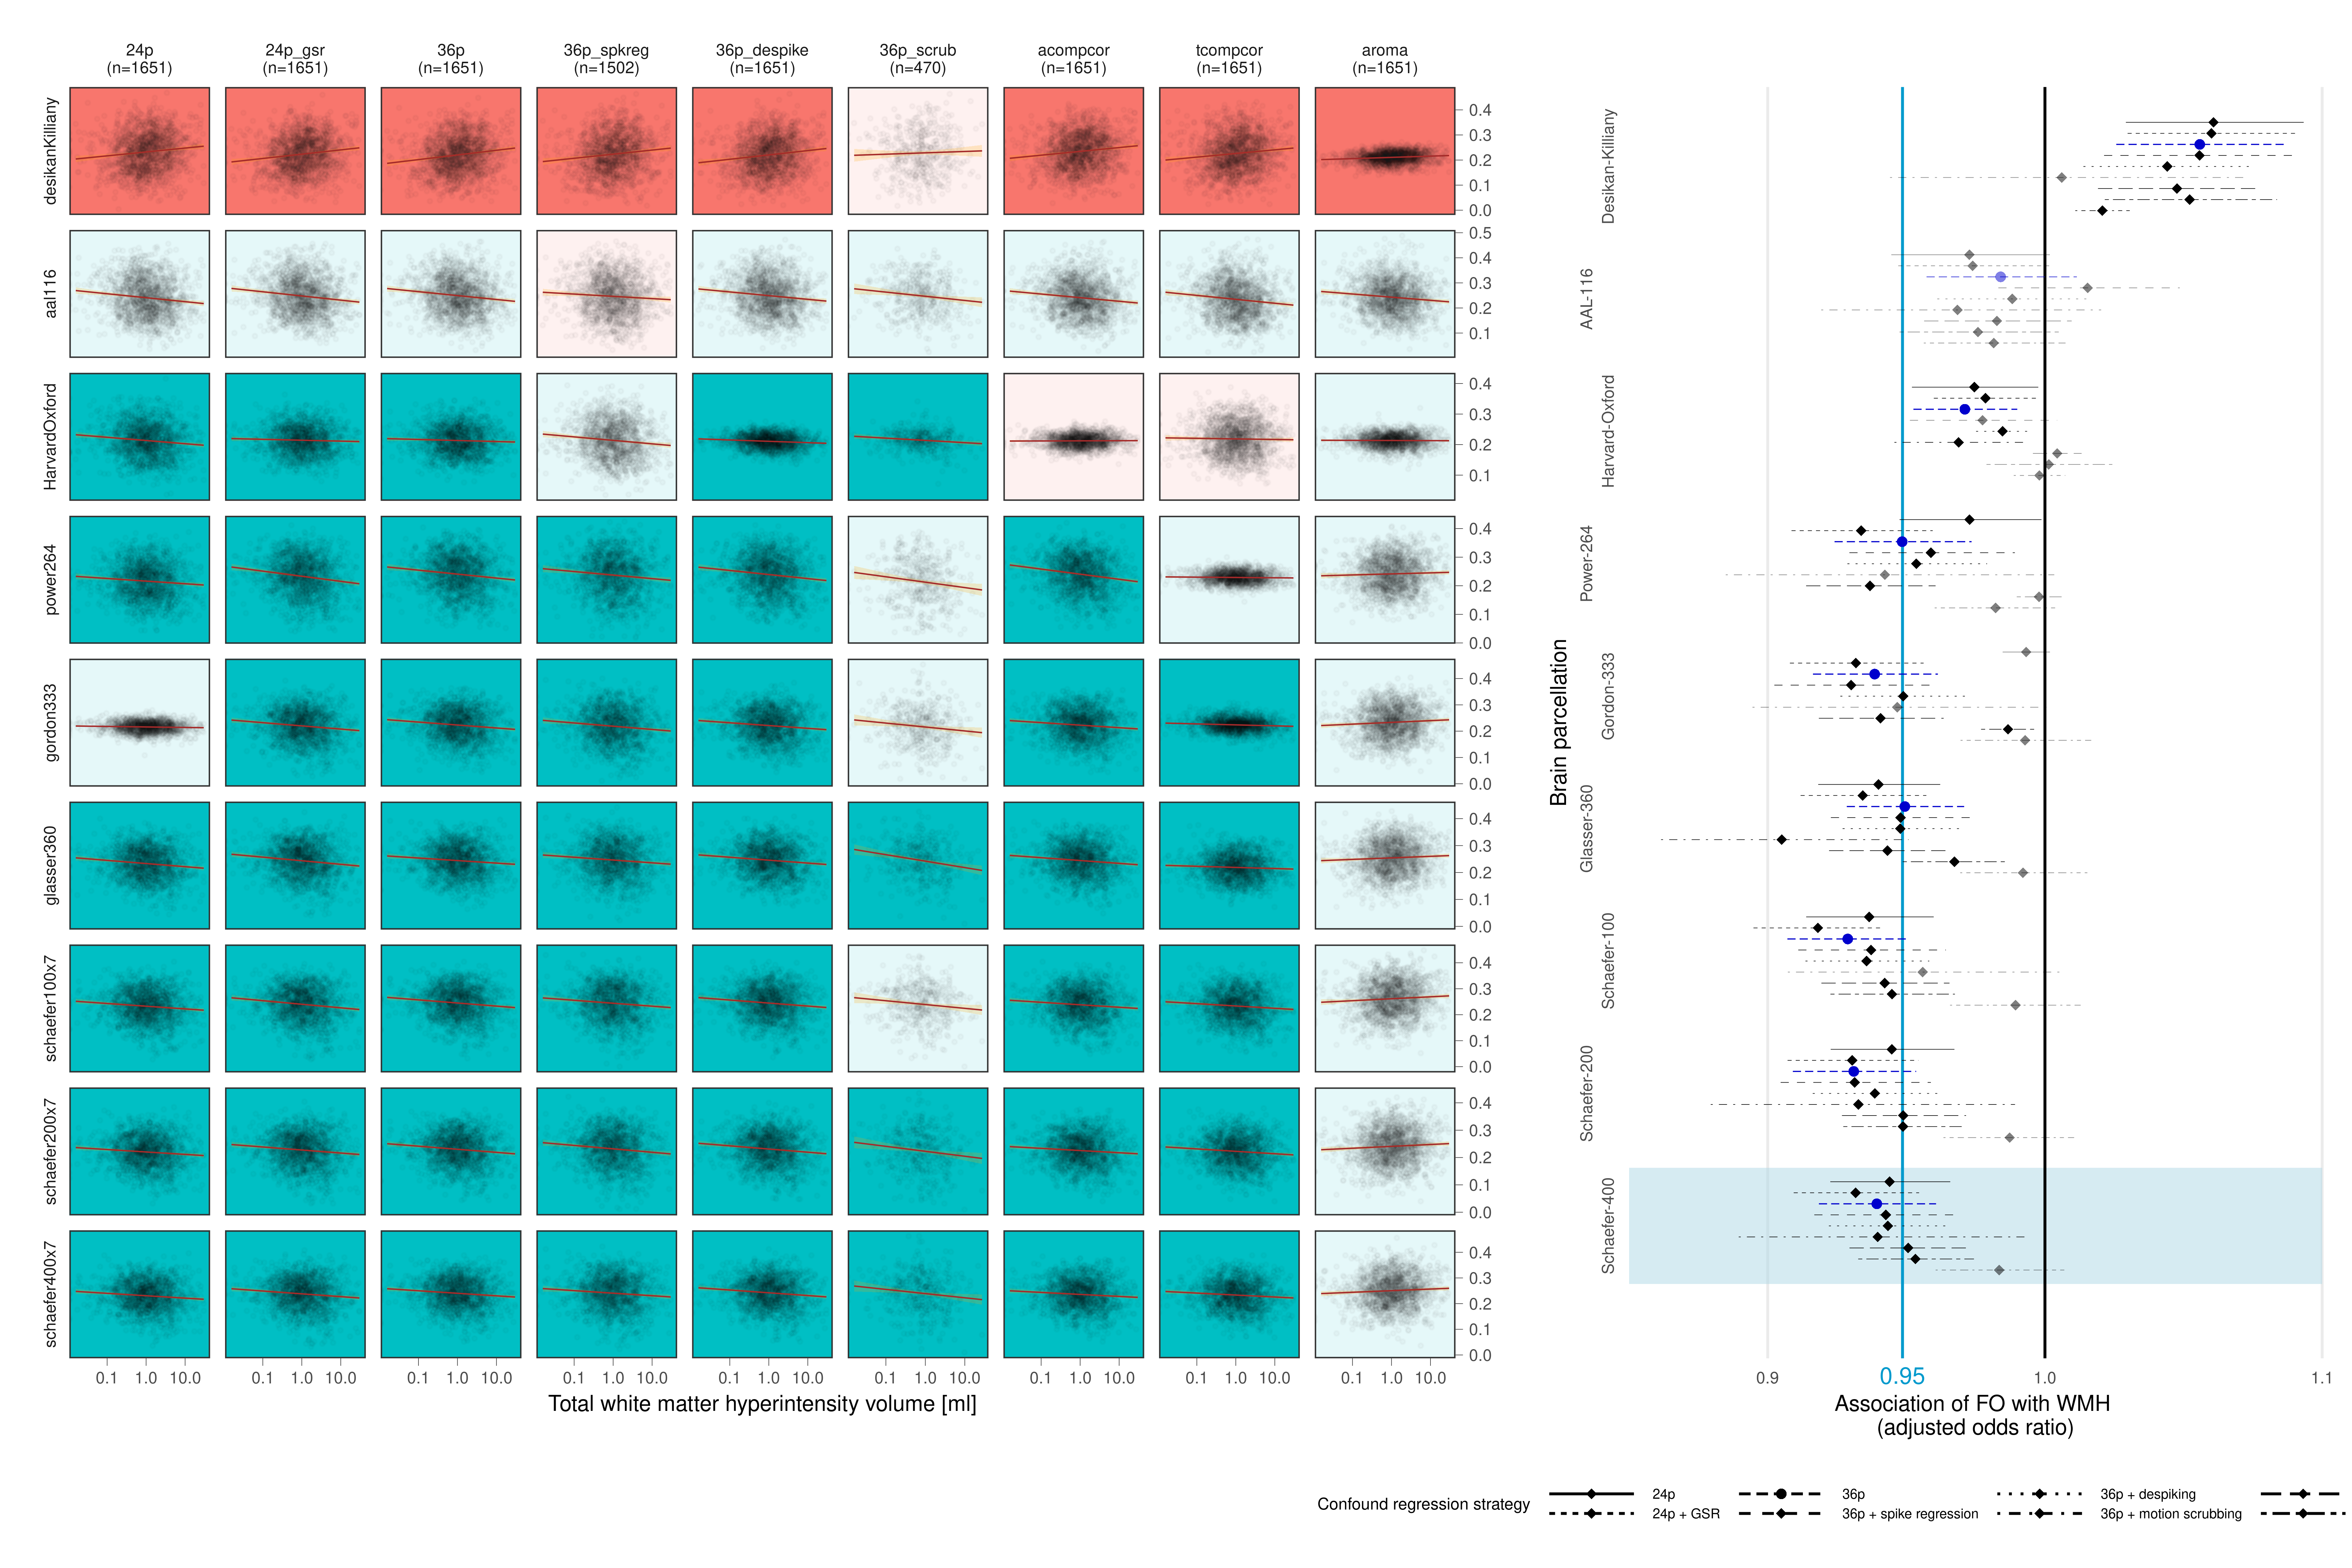
\includegraphics[width=\linewidth]{./../analysis/code/R/pipeline_files/figure-html/regWMHvsFOplot-1.png}
    \caption{On the left, scatter plots of average fractional occupancies in high-occupancy states against WMH volume on a logarithmic scale (base 10 for easier visualization) for different combinations of confound regression strategies and brain parcellations. Linear regression lines indicate the direction of the unadjusted association between log(WMH) and occupancy. Background color of individual panels indicates the direction of the association after adjustment for age, sex and zero WMH volume (green, negative; red, positive). A pale background indicates that the association between log(WMH) and average occupancy is not statistically different from zero. On the right, the same information is shown using point estimates and \qty{95}{\percent} confidence intervals for the adjusted odds ratio of the association.}
    \label{fig:refWMHvsFO}
\end{figure}

The secondary finding of an association between greater TMT-B times and lower fractional occupancy was similarly robust with 12/81 statistically significant negative and no statistically significant positive associations.

\subsection{Acknowledgment}
This preprint was created using the LaPreprint template (\url{https://github.com/roaldarbol/lapreprint}) by Mikkel Roald-Arb\o l \textsuperscript{\orcidlink{0000-0002-9998-0058}}.

\subsection{Disclosure}
The authors of this article declare that they have no financial conflict of interest with the content of this article.

%\subsection{Author contributions}
% According to https://journals.biologists.com/jeb/pages/author-contributions

\printbibliography

% DON'T EDIT. If "endfloat" option is enabled all floats appear before appendices
\if@endfloat\clearpage\processdelayedfloats\clearpage\fi 


%%%%%%%%%%%%%%%%%%%%%%%%%%%%%%%%%%%%%%%%%%%%%%%%%%%%%%%%%%%%
%%% SUPPLEMENTARY MATERIAL / APPENDICES
%%%%%%%%%%%%%%%%%%%%%%%%%%%%%%%%%%%%%%%%%%%%%%%%%%%%%%%%%%%%
%% Sadly, we can't use floats in the appendix boxes. So they don't "float", but use \captionof{figure}{...} and \captionof{table}{...} to get them properly caption.
% \begin{appendix}

% \begin{appendixbox}\label{app:ttt}
%     \section{Supplementary results}
\subsection{Deep and periventricular WMH}
Here we present, in analogy to \Cref{fig:mv}, the results of the multiverse analyses of the association between cSVD burden, FO of DMN-related states, and executive function, when cSVD is operationalized as the volume of deep or periventricular white matter hyperintensities, respectively.

    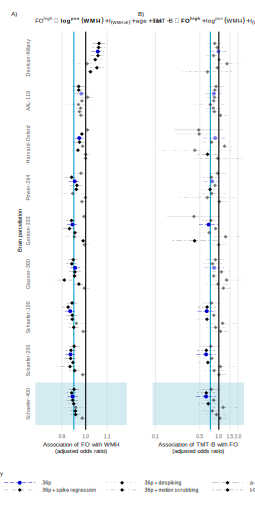
\includegraphics[width=\linewidth]{./../analysis/derivatives/Figures/Fig3deep.png}
    \captionof{figure}{\textbf{Multiverse analysis, deep WMH}}

    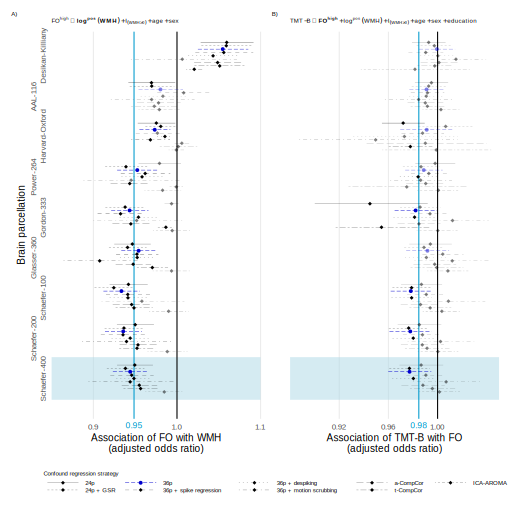
\includegraphics[width=\linewidth]{./../analysis/derivatives/Figures/Fig3peri.png}
    \captionof{figure}{\textbf{Multiverse analysis, periventricular WMH}}

\subsection{Motion parameters}
We also present, in analogy to \Cref{tab:hyp1,tab:hyp2}, regression tables for the association between time spent in DMN-related brain states (FO) and WMH volume, and between TMT-B and FO, adjusted for DVARS, RSMD and framewise displacement, in addition to age, sex and, in the latter case, years of education.

    \centering
    \setlength{\LTpost}{0mm}
    \begin{longtable}{lccc}
    \toprule
    & Estimate & P & 95\%-CI \\ 
    \midrule
    Intercept & 0.32 & <0.0001 & 0.28 -- 0.36 \\ 
    WMH, per 5.1-fold increase\textsuperscript{1} & 0.96 & 0.0004 & 0.94 -- 0.98 \\ 
    Age, per 10 years & 1.01 & <0.0001 & 1.00 -- 1.01 \\ 
    Female sex & 1.11 & <0.0001 & 1.08 -- 1.15 \\ 
    $\mathbf{1}_{\{\operatorname{WMH=0}\}}$ & 0.91 & 0.3552 & 0.74 -- 1.11 \\ 
    DVARS & 0.98 & <0.0001 & 0.98 -- 0.99 \\ 
    RMSD & 28.29 & 0.0055 & 2.67 -- 299.84 \\ 
    Framewise displacement & 0.16 & 0.0112 & 0.04 -- 0.66 \\ 
    \bottomrule
    \end{longtable}
    \textsuperscript{1} Interquartile ratio $2.37/0.468=5.06$
    \captionof{table}{Association between time-spent in high-occupancy DMN-related brain states and WMH volume adjusted for age, sex, and \textbf{motion parameters}}
    

    \centering
    \setlength{\LTpost}{0mm}
    \begin{longtable}{lccc}
    \toprule
    & Estimate & P & 95\%-CI \\ 
    \midrule
    Intercept & 46.83 & <0.0001 & 36.74 -- 59.72 \\ 
    $\operatorname{FO}^{\text{high}}$, per 5\%  & 0.71 & 0.0718 & 0.49 -- 1.03 \\ 
    WMH, per 5.1-fold increase\textsuperscript{1}  & 1.01 & 0.3414 & 0.98 -- 1.04 \\ 
    Age, per 10 years & 1.02 & <0.0001 & 1.01 -- 1.02 \\ 
    Female sex & 1.00 & 0.8171 & 0.96 -- 1.04 \\ 
    Education, per year  & 0.97 & <0.0001 & 0.97 -- 0.98 \\ 
    $\mathbf{1}_{\{\operatorname{WMH=0}\}}$ & 0.96 & 0.7581 & 0.73 -- 1.29 \\ 
    DVARS & 1.01 & 0.0001 & 1.00 -- 1.01 \\ 
    RMSD & 0.31 & 0.4695 & 0.01 -- 7.45 \\ 
    Framewise displacement & 1.08 & 0.9322 & 0.16 -- 7.13 \\ 
    \bottomrule
    \end{longtable}
    \textsuperscript{1} Interquartile ratio $2.37/0.468=5.06$
    \captionof{table}{Association between TMT-B and time spent in high-occupancy DMN-related brain states adjusted for age, sex, WMH volume and years of education, and \textbf{motion parameters}}
% \end{appendixbox}

% \begin{appendixbox}
%     \input{src/supplementary/resources.tex}
% \end{appendixbox}

% \end{appendix}


%%%%%%%%%%%%%%%%%%%%%%%%%%%%%%%%%%%%%%%%%%%%%%%%%%%%%%%%%%%%
%%% ARTICLE END
%%%%%%%%%%%%%%%%%%%%%%%%%%%%%%%%%%%%%%%%%%%%%%%%%%%%%%%%%%%%

\end{document}
